\subsection{Problem Statement}
\label{sec:problem}

%\ana{Ishaq? Basically, define sequential schedule, then define an equivalent parallel schedule. A parallel schedule is equivalent if it preserves def-use relations in sequential schedule, or in other words, schedules def ahead of the use. Problem is to minimize cost of Parallel schedule.}

As mentioned earlier, at the lowest level, we have two types of MPC instructions (also called \emph{gates} in similar works) 1) local/non-interactive instruction (i.e. an addition instruction $A$) and 2) remote/interactive instruction (i.e. a multiplication instruction $M$). %Each instruction in the program is either an $A$-instruction or an $M$-instruction.

% Let the cost of a single \add ~instruction be given by a monotonically decreasing $f(n)$, where the argument $n$ is the number of \add ~instructions being executed in parallel. Similarly the cost of a single \mul ~is given by a monotonically decreasing function $g(n)$.

Given a serial schedule (a linear graph) of an MPC program i.e. a sequence of instructions $S := (S_1; \dots; S_n)$, where $S_i \in \{A, M\}, 1 \leq i \leq n$, and a def-use dependency graph $G(V, E)$ corresponding to $S$, our task is to construct a parallel schedule (another linear graph) $P := (P_1; \dots; P_m)$ observing the following conditions:

\begin{enumerate}
    \item All $P$'s consist of MPC instructions of the same kind, e.g., all MUL, or ADD, etc. 
    \item Def-use dependencies of the graph $G(V, E)$ should be preserved i.e. if instructions $S_i, S_j, i < j$ form a def-use i.e. an edge exists from $S_i$ to $S_j$ in $G$, then they can only be mapped to $P_{i'}, P_{j'}$ such that $i' < j'$.
\end{enumerate}

\paragraph{Correctness} Correctness of $P$ is guaranteed by definition. Preserving def-use \emph{dependencies} means the computed function remains the same in both $S$ and $P$.

In order to benefit from parallelization/amortization, we must schedule two or more $A$-instructions in the same parallel node (or two or more $M$-instructions in the same parallel node). Recall that we also assume that scheduling $A$-instructions in parallel with $M$-instruction does not benefit from amortization\footnote{this is not strictly true, but assuming it, e.g. as in \cite{Ishaq2019, Demmler2015ABYA, Mohassel2018}, helps simplify the problem.}. It incurs the exact same cost as scheduling the $A$-instructions in a node $P_A$, scheduling the $M$-instructions in a node $P_M$, and having $P_A$ precede $P_M$ in the parallel schedule. We use the following cost model:

%\begin{enumerate}
%    \item $A$ costs $\alpha$ units and $M$ costs $\beta$ unites.
%    \item There is unlimited bandwidth i.e. a single $A$-instruction (or $M$-instruction) costs as much as $N$ amortized $A$-instructions (or $M$-instructions), concretely either $\alpha$ unites or $\beta$ units.
%\end{enumerate}

The cost of schedule $S$ is
\begin{equation}
    \mathit{cost}(S) = \sum_{i=1}^n \mathit{cost}(S_i)
\end{equation}

where $cost(S_i) = \alpha$ or $\beta$. %if $S_i$ is an $A$-instruction and $cost(S_i) = \beta$ if $S_i$ is an $M$-instruction. 
Similarly, the cost of schedule $P$ is

\begin{equation}\label{eq_par_schedule_cost}
    \mathit{cost}(P) = \sum_{i=1}^m \mathit{cost}(P_i)
\end{equation}

Each $P_i$ may contain multiple instructions, and $\mathit{cost}(P_i)$ is amortized.
Thus, according to our model $\mathit{cost}(P_i) = \alpha_\mathit{fix} + |P_i|\alpha_\mathit{var}$ if $P_i$ stores $\alpha$-instructions, 
or $\mathit{cost}(P_i) = \beta_\mathit{fix} + |P_i|\beta_\mathit{var}$ if it stores $\beta$-instructions.
%if $P_i$ consists of $A$-instructions only, it is $\beta$ if $P_i$ consists of $M$-instructions only, and it is $(\alpha + \beta)$ if $P_i$ mixes $A$-instructions and $M$-instructions. 
Our goal is to construct a parallel schedule $P$ that reduces the program cost (when compared to cost of $S$), possibly an optimal schedule. 
Originally we hoped that the problem is simper and computation of the optimal schedule is tractable. Unfortunately, the optimal schedule turns out to be NP-hard via a reduction 
to the Shortest Common Supersequence problem.

% \paragraph{Cost Comparison} For the sequential schedule $\mathcal{S}$ consisting of $L$ local and $R$ remote instructions, the total cost is $\mathit{cost}(\mathcal{S}) = L \cdot f(1) + R \cdot g(1)$. In the extreme case where all $L$ and all $R$ instructions can be parallelized, the cost of $\mathcal{P}$ is $\mathit{cost}(\mathcal{P}) = L \cdot f(L) + R \cdot g(R)$. Since both $f$ and $g$ are monotonically decreasing, $\mathit{cost}(\mathcal{P}) < \mathit{cost}(\mathcal{S})$. Cost of all other parallel schedules lies between the extremes of $\mathit{cost}(\mathcal{S})$ and $\mathit{cost}(\mathcal{P})$.

Note that we consider a linearized MPC schedule $S$ above for ease of exposition only. In our tool-chain we use an MPC Source control flow graph (CFG) $G'(V', E')$ along with def-use graph $G(V,E)$ to construct $P$. %The argument becomes slightly more involved when dealing with a graph $G'$ that may contain cycles.

\subsection{Scheduling is NP-hard}
\label{sec:np}

To prove that optimal scheduling is an NP-Hard problem, we consider the following convenient representation. An MPC program is represented as a set of sequences $S = \{S_1, \dots, S_n\}$. Each element $S_i \in S$ is a tuple. The items of the tuple $S_i$ are operations, i.e. $A$ or $M$ instructions, that have to be executed in order (operations depend on previous operations i.e. $S_i[j], j > 1$ depends $S_i[j-1]$). However, the sequences $S_i, 1 \leq i \leq n$ themselves, can overlap each other in any way i.e. distinct sequences can be executed in parallel. We argue that an MPC program can be transformed into such collection of sequences by traversing the circuit for each pair of input and output values. \ishaq{I am not sure how this will be done, see \cref{fig:sequence_construction}}

As an example, consider the MPC program consisting of the following three sequences, all made up of two distinct $\alpha$-instructions $M_1$ and $M_2$. The right arrow indicates a def-use \emph{dependence}, meaning that the source node must execute before the target node: 

\begin{enumerate}
    \item $M_1 \rightarrow M_2 \rightarrow M_1$
    \item $M_1 \rightarrow M_1 \rightarrow M_1$
    \item $M_2 \rightarrow M_1 \rightarrow M_2$
\end{enumerate} 

%A \emph{schedule} $P: (P_1 ; P_2 \dots ; P_m)$ is such that for each sequence $S_i$ in the set, if $S_i[j]$ precedes $S_i[j']$ in $S_i$ then $S_i[j]$ is scheduled in node $P_\ell$, $S_i[j']$ is scheduled in node $P_{\ell'}$, and $P_\ell$ precedes $P_{\ell'}$ in $P$. 

% The cost of a schedule $P$ is 

% \begin{equation}
%     \mathit{cost}(P) = \sum_{i=1}^k \mathit{cost}(P_i)
% \end{equation}

% where $\mathit{cost}(P_i) = \alpha$ if $P_i$ consists of $A$-instructions only, it is $\beta$ if $P_i$ consists of $M$-instructions only, and it is $(\alpha + \beta)$ if $P_i$ mixes $A$-instructions and $M$-instructions. 

The problem is to find a schedule $P$ with \emph{minimal cost}. For example, a schedule with minimal cost for the sequences above is 

$$ 
M_1(1), M_1(2) \; ;\; M_1(2) \; ; \; M_2(1), M_2(3) \; ; \; M_1(1), M_1(2), M_1(3) \; ; \;  M_2(3)
$$

The parentheses above indicate the sequence where the instruction comes from: (1), (2), or (3). 
Cost of schedule $P$ is computed using \cref{eq_par_schedule_cost} above and it amounts to $5\alpha_\mathit{fix} + 9\alpha_\mathit{var}$.

The problem of finding a schedule $P$ with a minimal $cost(P)$ is shown to be NP-Hard problem, as it can be reduced to the problem of finding a \emph{shortest common supersequence}, a known NP-Hard problem\cite{Maier1978, Vazirani2010}. The shortest common supersequence problem is as follows: {\it given two or more sequences find the the shortest sequence that contains all of the original sequences.} This can be solved in $O(n^k)$ time, where $n$ is the cardinality of the longest sequence and $k$ is the number of sequences. For our problem $n$ is the maximum length of a sequence and $k$ is the number of total number of sequences. We can immediately see that the optimal schedule is the shortest schedule, since the shortest schedule minimizes the fixed cost while the variable cost remains the same.

\ana{This paragraph needs work.} To formalize the reduction, suppose $P$ is a schedule with minimal cost (computed by a black-box algorithm). 
%We can derive a schedule $P'$ with the same cost as $P$, by mapping each mixed node $P_i \in P$ to two consecutive nodes in $P'$: an $A$-instruction node followed by an $M$-instruction node. 
Clearly, $P'$, which now is a sequence of $M_1$ and $M_2$ nodes, is a supersequence of each sequence $S_i$, i.e., $P'$ is a common supersequence of $S_1 \dots S_n$. It is also a shortest common supersequence. 
%To see this, let $X$ and $Y$ denote, respectively, the number of $A$ and $M$ nodes in $P'$. 
The cost of $P$, is $L\alpha_\mathit{fix}+N\alpha_\mathit{var}$ where $L$ is the length of $P$ and $N$ is the total number of instructions across all sequences. %$X \cdot \alpha + Y \cdot \beta$. 

Now suppose, there exists a shorter common supersequence $P'$. 
that consists of $X'$ nodes of type $A$-instructions $Y'$ nodes of type $M$-instructions. Since $P''$ is shorter than $P'$, therefore $X' + Y' < X + Y$, and $X' \cdot \alpha + Y' \cdot \beta < X \cdot \alpha + Y \cdot \beta$ i.e. $\mathit{cost}(P'') < \mathit{cost}(P')$. But $\mathit{cost}(P') = \mathit{cost}(P)$ and $\mathit{cost}(P)$ is the optimal cost.  Therefore $\mathit{cost}(P'') < \mathit{cost}(P')$ is contradiction and no such $P''$ exists. \qed

\begin{comment}
\subsection{Loud Thinking}
\ishaq{I will delete this section after we have decided on how to handle various issues raised in this section}.

\begin{figure}
  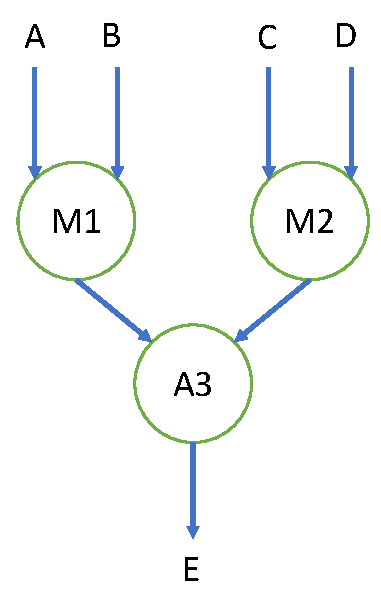
\includegraphics[width=0.6\linewidth]{./figs_paper_SIMD/sequence_construction.pdf}
  \caption{How do we construct sequences from this circuit?} 
  \label{fig:sequence_construction}
\end{figure}

The more realistic cost model is as under:
\begin{enumerate}
    \item The cost of an $A$-instruction is given by a function $\alpha(\cdot)$ where the only parameter to the function is the number of $A$ instructions that will be executed in parallel.
    \item Similarly, the cost of an $M$-instruction is given by function $\beta(\cdot)$.
    \item Both $\alpha$ and $\beta$ are amortization function e.g. $\alpha(n) \leq \alpha(\ell) + \alpha(m); n = \ell + m$. Same condition applies for $\beta$.
\end{enumerate}

\begin{figure}
  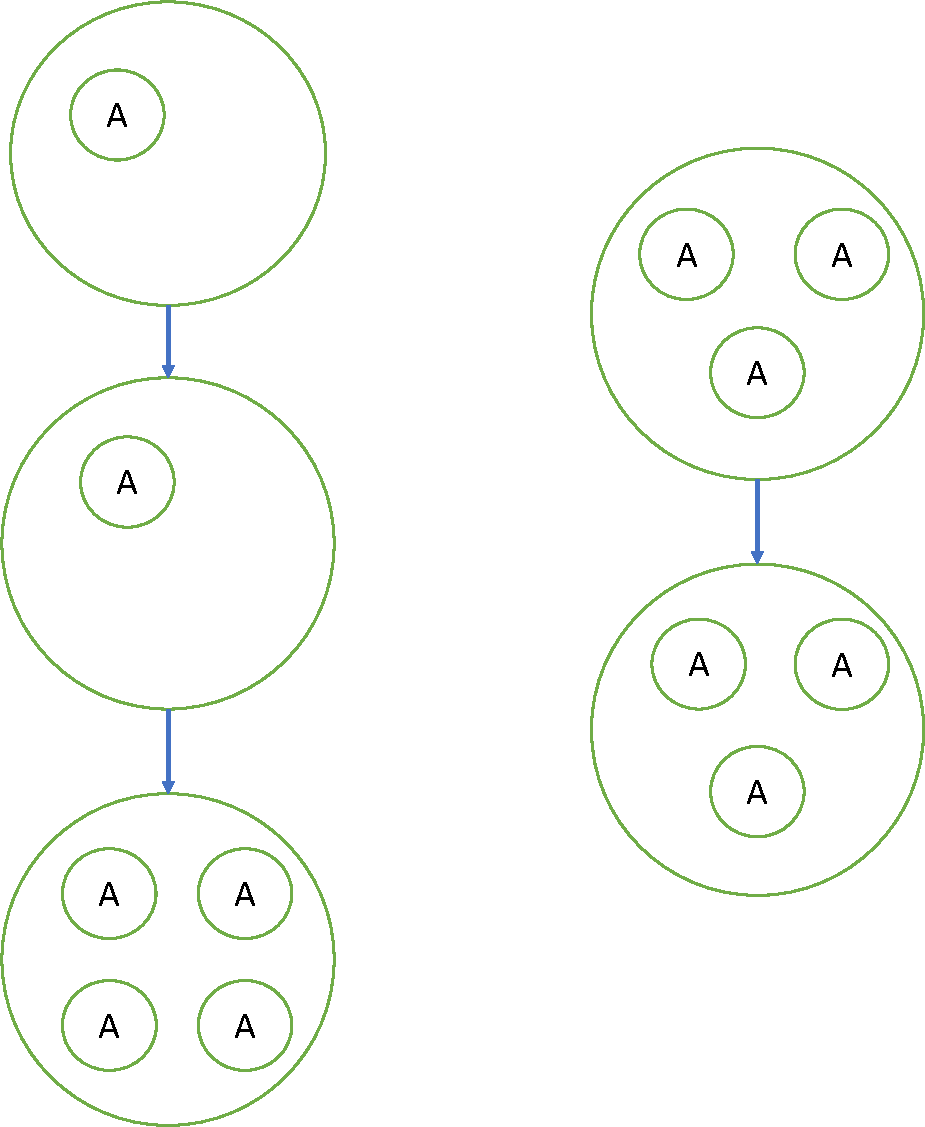
\includegraphics[width=0.6\linewidth]{./figs_paper_SIMD/cost_inequality.pdf}
  \caption{It is unclear whether right super sequence cost less/more/the-same as left one.} 
  \label{fig:cost_comparison}
\end{figure}

I am not using this cost model (for now) because NP-Hardness proof is tricky (see \cref{fig:cost_comparison}). Consider a super sequence that has nodes (of only one type) with following weights: $SS_1 = (1, 1, 4)$ where $Length(SS_1) = 3$ and $cost(SS_1) = \alpha(1) + \alpha(1) + \alpha(4)$.

Using $\alpha(4) \leq \alpha(1) + \alpha(3)$, we can say 

\begin{equation}\label{ineq_cost_1}
    \alpha(1) + \alpha(1) + \alpha(4) \leq \alpha(1) + \alpha(1) + \alpha(1) + \alpha(3)
\end{equation}

Now suppose, for the same schedule, another super sequence with weights $SS_2 = (3, 3)$ exists, $Length(SS_2) = 2$ and $cost(SS_2) = \alpha(3) + \alpha(3)$. Using $\alpha(3) \leq \alpha(1) + \alpha(1) + \alpha(1)$, we can say

\begin{equation}\label{ineq_cost_2}
    \alpha(3) + \alpha(3) \leq \alpha(1) + \alpha(1) + \alpha(1) + \alpha(3)
\end{equation}

The problem is that while RHS is the same in \cref{ineq_cost_1} and \cref{ineq_cost_2}, we cannot say anything about the relationship between their LHS. It could be possible that cost of $SS_2$, LHS of  \cref{ineq_cost_2}, is more than cost of $SS_1$, LHS of \cref{ineq_cost_1}. Thus, we have a shorter super sequence $SS_2$ that does not contradict that the optimality of the schedule used to generate $SS_1$.
\end{comment}